\documentclass[conference]{IEEEtran}

\usepackage[english]{babel}
\usepackage{array}
\usepackage{multirow}
\usepackage{csquotes}
\usepackage{fixltx2e}
\usepackage{subfigure}
\usepackage{graphicx}

%common abbreviations
\newcommand{\etal}{{\it et al.}}
\newcommand{\etc}{{\it etc.}}
\newcommand{\ie}{\emph{i.e.}}
\newcommand{\eg}{{\em e.g.}}

\begin{document}

\title{DC4Cities: Better Usage of the Renewable Energies in Data Centres}

\author{\IEEEauthorblockN{Corentin Dupont}
\IEEEauthorblockA{Create-Net\\
Trento, Italy\\
Email: cdupont@create-net.org}
\and
\IEEEauthorblockN{Fabien Hermenier}
\IEEEauthorblockA{Univ. Nice Sophia Antipolis\\
CNRS, I3S, UMR 7271,\\
France\\
Email: fabien.hermenier@unice.fr}}

\maketitle

Data centre are a key part of the ICT chain.
The energy consumed by them in 2010 accounted for between 1.1\% and 1.5\% of the total electricity consumed worldwide~\cite{Koomey2011}, making of data centre energy management an important challenge for researchers.
With the recent adoption of renewable energies to power data centres~\cite{parasol-sigplan2013}, the research community enlarges its vision to associate with purely \emph{quantitative} energy consumption reduction, the notion of \emph{quality} of the energy consumed, \ie\ the capacity to rely as much as possible on sustainable power sources.
Differently from non-renewable energy sources, the availability of renewable energies is very volatile and time dependent: \eg\ solar power is obtainable only during the day, and is subject to variations due to the meteorological conditions.
The goal in this case is to shift the workload of running applications, according to the forecasted availability.

\begin{figure}[ht!]
  \centering
  \subfigure{
     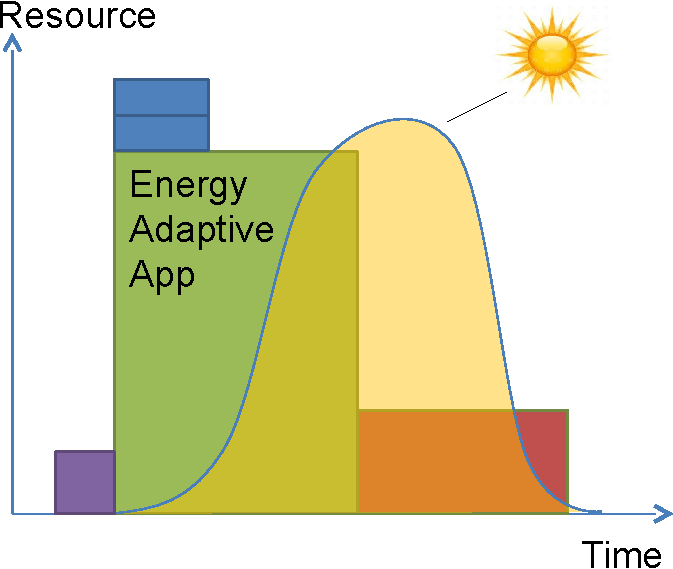
\includegraphics[width=0.42\linewidth]{figs/noadapt}
  }     
  \subfigure{
     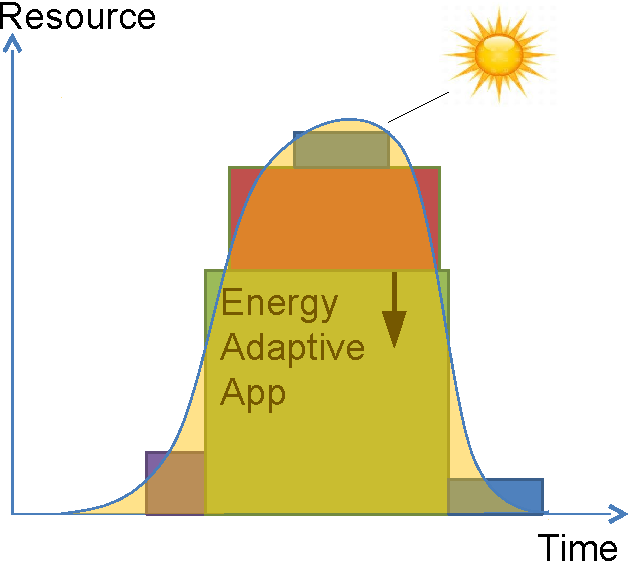
\includegraphics[width=0.40\linewidth]{figs/adapt}
  }     
  \caption{Adapting applications for a better usage of renewable energies}
  \label{fig:adapt}
  \vspace{-1em}
\end{figure}

In our scenario, an entity external to the data centre, called the Energy Management Authority (EMA), is able to set high-level energy and power objectives for the data centre.
For example, an objective can be: \enquote{at least 80\% of the data centre energy consumption has to be generated from renewable energy sources}.
To translate these high-level objectives into concrete actions performed in the data centre, our platform receives forecasts regarding the amount of available power and the energy source mix of its electricity inputs.
These forecasts are either provided directly by the power suppliers or created by algorithms which use environmental and historical data to predict future renewable energy generation.
Having both workload estimations for the different running applications~\cite{Kansal2008} and the energy forecasts, our platform is able to assign specific power budgets to the different applications.
%The applications, in turn, choose their specific working mode to respect the power budget and the SLAs.

In order to run the applications in a data centre while respecting this power budget, we introduce the concept of Energy Aware Software Controller (EASC).
The EASC is able to: (i) manage elasticity and scalability of multi-tier applications according to their energy footprint (\emph{energy-awareness}); (ii) inject mechanisms in the single applications to negotiate energy usage according to energy constraints (\emph{energy-adaptiveness}).

%initial concepts of DC4Cities, a FP7 project that aims to make data centres more efficient according to the availability of renewable energies.
The EASC implements workload scheduling techniques that can reconfigure the applications according to the power budgets (see Figure~\ref{fig:adapt}).
An EASC is attached to each specific application running in the data centre and receives a different power budget, corresponding to the expected power consumed by the controlled application.
The EASC is then proposing several plans to perform the application's tasks, within the limits of its SLA.
Those plans can be influenced using two weighted parameters: the aggressiveness and the eagerness.
The aggressiveness controls the possibility for the application to consume more or less aggressively the renewable energies.
For example, at a high aggressivity level the application will run at the highest performance level when renewable energies are available, and at the lowest performance when they are not.
The eagerness controls the necessity for an application to complete its tasks more or less early.
A low eagerness allow to be more flexible with regard to the scheduling of the applications tasks during the period of availability of the renewable energies.
The EASCs are coordinated by the central component of our platform prototype.
This central component coordinates the EASCs and selects the correct plan for each EASC, in order to optimize their combination.

A specific EASC has been designed to control the IaaS layer of modern data centres. It is used to consolidate the VMs that are running the applications, in order to free up some servers and switch them off when there is a low percentage of renewable energies.
Similarly, an EASC for the PaaS layer is used to scale up and down PaaS applications with regard to its tasks, SLA and energetic situation.

Our solution has been trialled in the data centre of the health agency of the province of Trento, Italy.
In this trial, the EASC was controlling a real application producing medical reports.
We used an SLA stating that the application should be able to create 780 reports per day at minimum.
Using our prototype, the percentage of renewable energy consumed by the data centre (called REN\%) went from 43.1\% up to 57.9\%. 


\section{Acknowledgments}
The authors would like to thank the EU FP7 project DC4Cities (grant agreement number 609304), and the consortium members.

\bibliographystyle{unsrt}
\bibliography{bibliography/central-bibliography} 

\end{document}

